\begin{titlepage}
  \symmetricalPage%
  \begingroup%
    %\tikzset{external/export=false}%%
    \begin{tikzpicture}[
        overlay,
        remember picture,
      ]
      \node[anchor=center] at ($(current page)+(-3.1,-5)$) {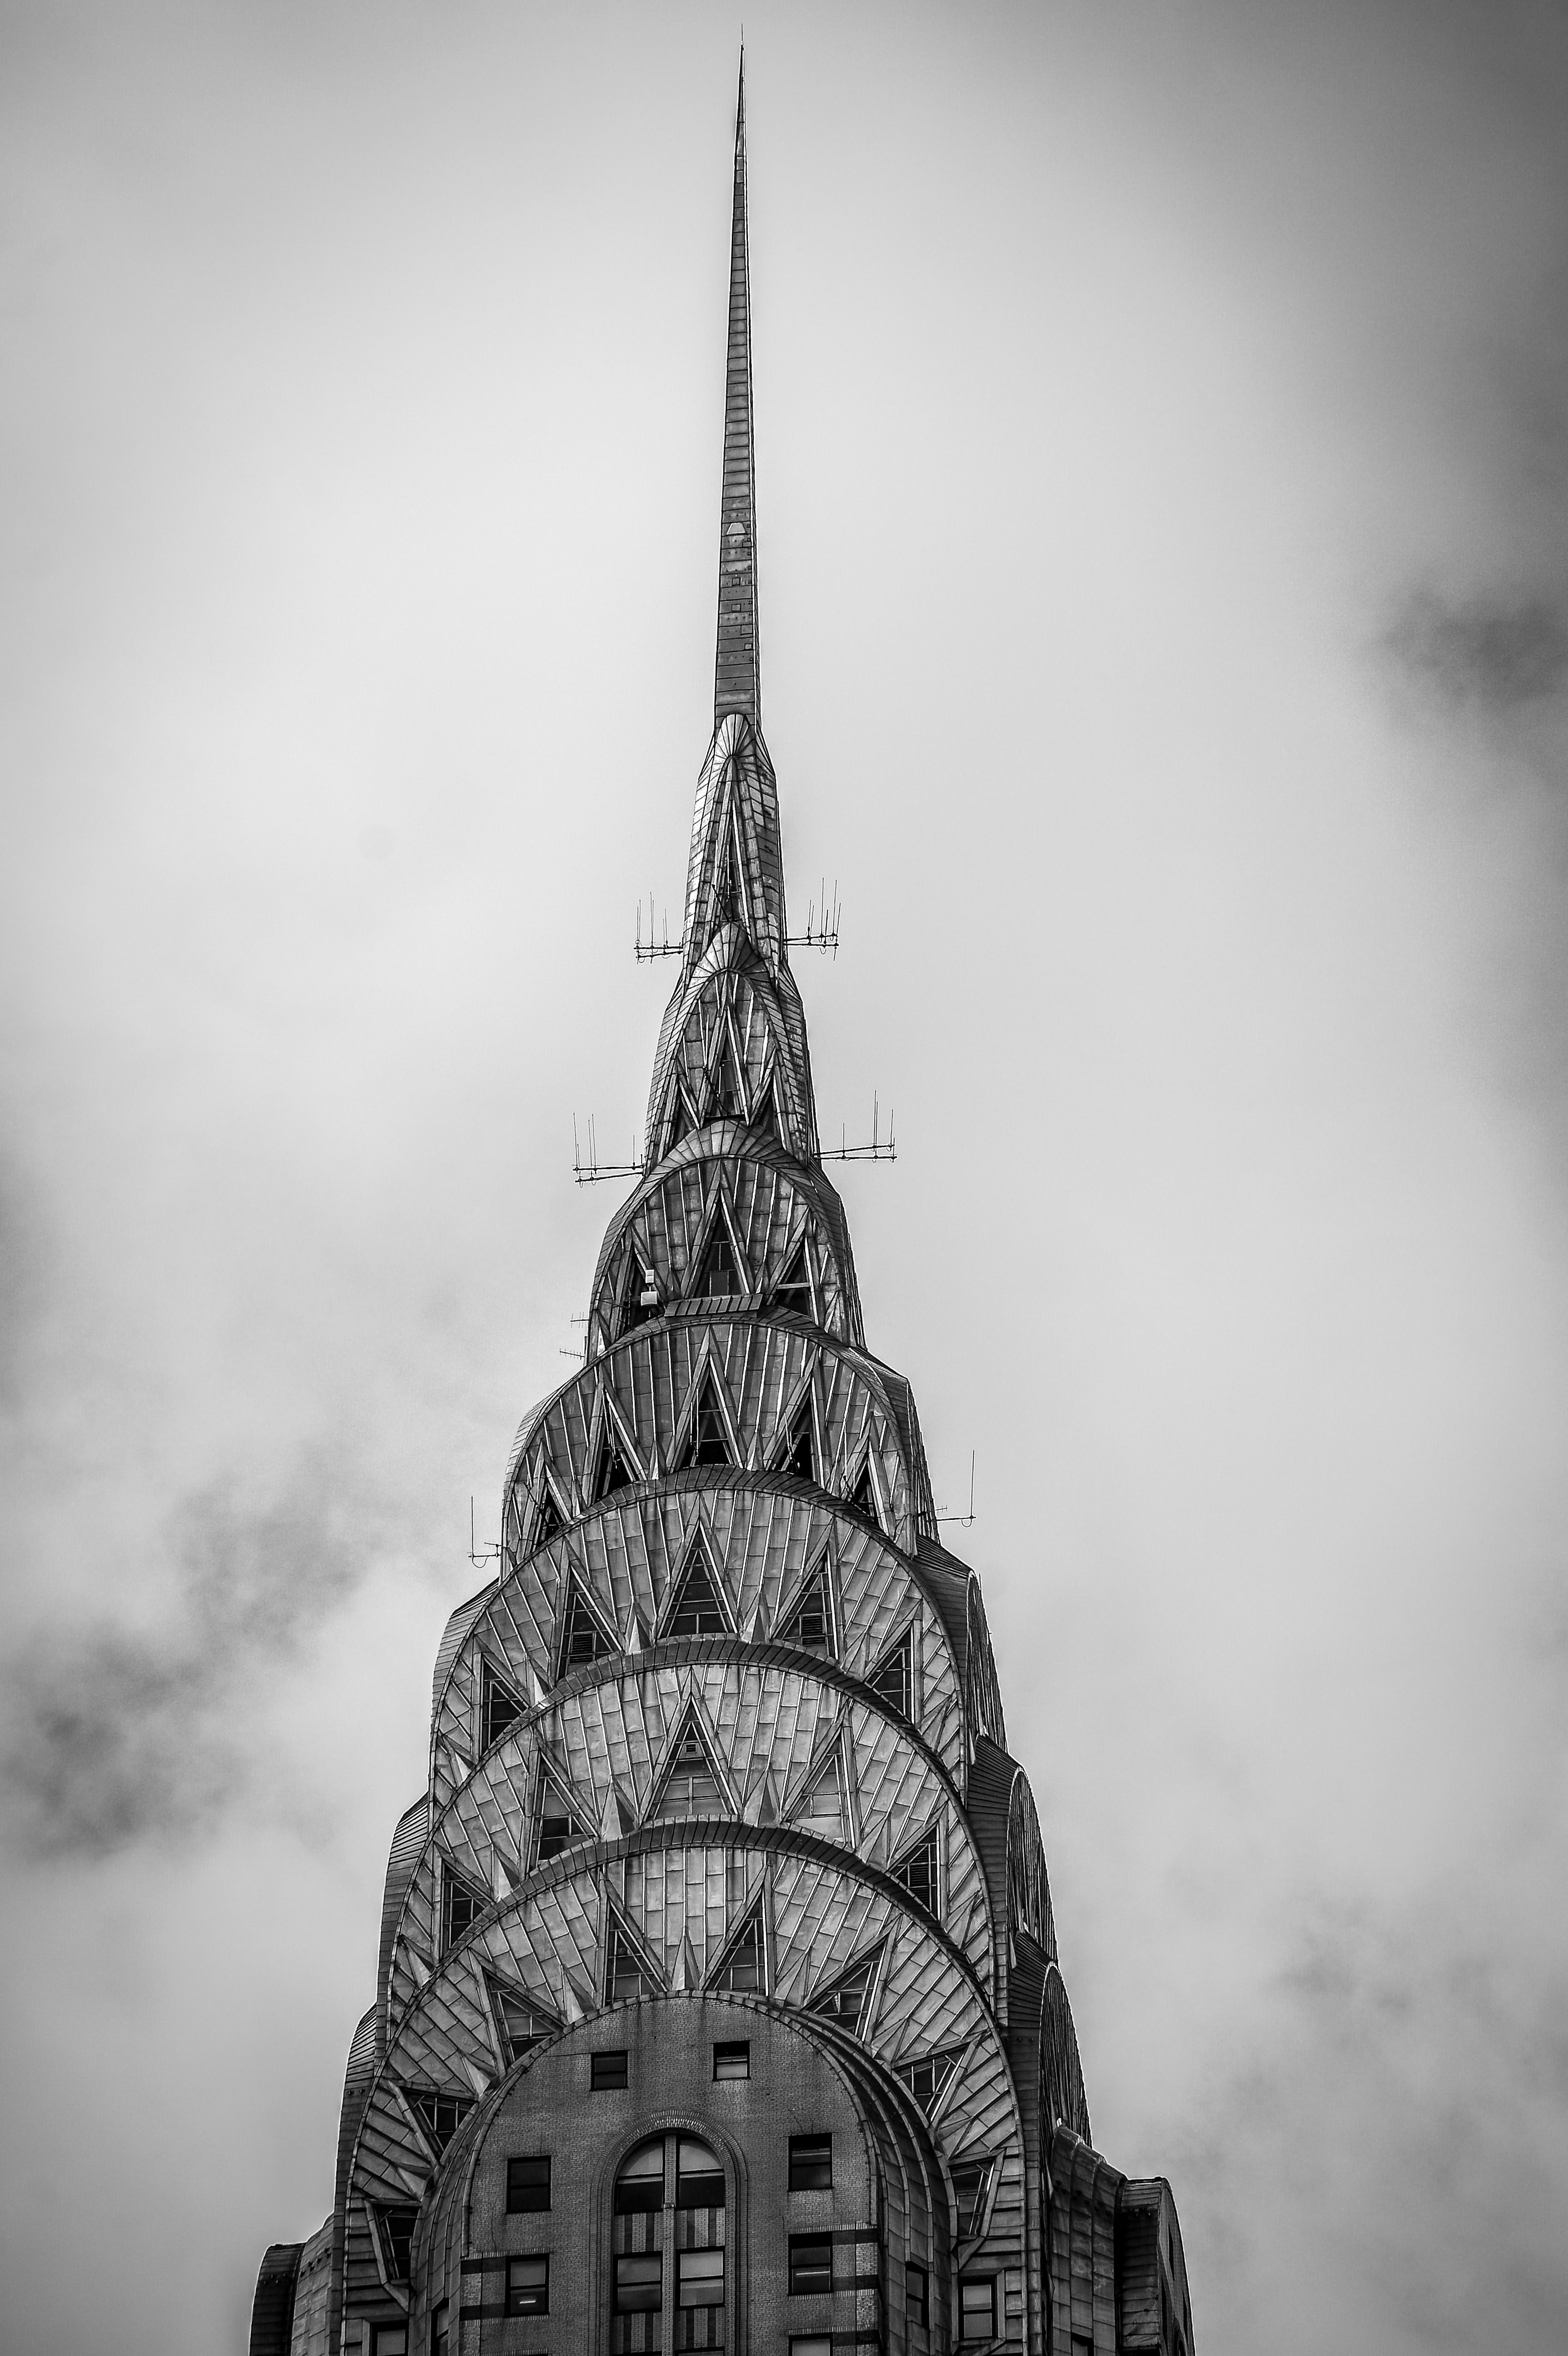
\includegraphics[width=1.3\paperwidth]{Images/Portada/FONDO.jpg}};
    \end{tikzpicture}
  \endgroup%
  %\sffamily%

  \vspace*{2cm}%
  \begingroup%
    \bfseries\flushright%
    % \scshape%
    \begingroup%
      \Huge%
      \color{black}
      \noindent\scalebox{2}{NOTAS DE}\\[10mm]
      \scalebox{2}{CÁLCULO III}\\[50mm]
    \endgroup%
    \begingroup%
      \bfseries\LARGE%
      \color{black}%
      ~\hfill\begin{tabular}{r}
          Sabino D. Castro\\[4mm]
          Antonio M. Mendoza
      \end{tabular}
      %~\hfill Sabino D. Castro\\[4mm]
      %~\hfill Antonio M. Mendoza
    \endgroup%
  \endgroup%

  \vfill%
  \noindent\parbox[b]{\linewidth-5cm}{%
    \begingroup%
      ~
    \endgroup%
  }%
  ~\hfill%
  \parbox[b]{3cm}{%
    
\includegraphics[width=\linewidth]{Images/Portada/LOGO.pdf}
  }
\end{titlepage}
\restoregeometry%

\newpage
\,

\newpage

\symmetricalPage%

\begin{tikzpicture}[remember picture,overlay]%
      \coordinate (A) at ($(current page.north)!.4!(current page.north east)$);
      \coordinate (B) at (current page.east);
      \coordinate (C) at (current page.north east);

      \filldraw[black] (A) -- (B) -- (C) -- cycle;
\end{tikzpicture}

\,
\vspace{3cm}
\begin{center}
\scalebox{4}{\textbf{CÁLCULO III}}\\
\,
\,\\
\scalebox{2}{\textbf{Cálculo de varias variables}}\\
\,\\
\,\\
\scalebox{1.3}{\textbf{Andrés Sabino Díaz Castro}}\\
\,\\
Profesor de matemáticas de la ESFM\\
\vspace{2cm}
\begin{center}
      \begin{tikzpicture}
            \node at (current page.center) {
\includegraphics[width=0.3\textwidth]{Images/Portada/POLITECNICO.pdf}}; % Logo de institución
      \end{tikzpicture}
\end{center}
\vfill
México, 2024
\end{center}

\restoregeometry%

\newpage
\,